\pgfplotsset{
	axis background/.style={fill=none},
	%tick style=mygrey2,
	%tick label style=mygrey2,
	grid=none,
	%xtick pos=left,
	%ytick pos=left,
	tick style={
		major grid style={style=white,line width=1pt},minor grid style=white,
%		major grid style={style=white,line width=1pt},minor grid style=mygrey3,
		%tick align=outside,
	},
	%minor tick num=4,
}

\begin{figure}[tb]
	\centering
	 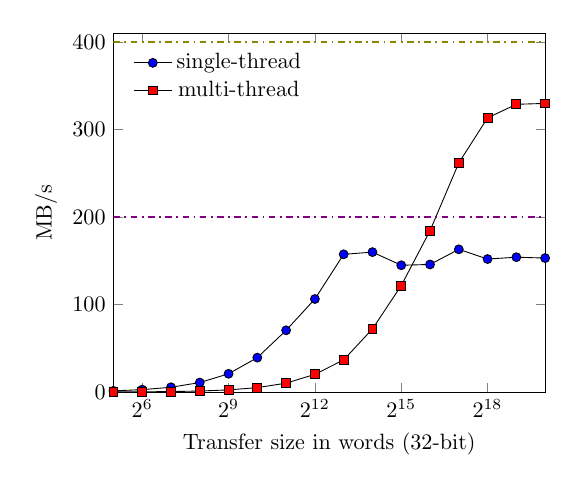
\begin{tikzpicture}[scale = 0.8]
	 \begin{axis}[
	 xmode=log,
	 log basis x={2},
	 xlabel=Transfer size in words (32-bit),
	 ymin=0,
	 ymax=410,
	 xmax = 1048576,
	 xmin = 32,
	 ylabel=MB/s,
%	 legend style={at={(0.3,0.8)},anchor=north}
	 legend pos=north west,
	 legend style={draw=none}
	 ]    

	\addplot [mark=*,mark options={fill=blue}] plot coordinates {
		(32,     1.4)
		(64,     2.8)
		(128,     5.5)
		(256,     10.9)
		(512,      20.9)
		(1024,     39.4)
		(2048,     70.6)
		(4096,     106.4)
		(8192,     157.5)
		(16384,    160.0)
		(32768,    145.0)
		(65536,    145.9)
		(131072,    163.2)
		(262144,    152.1)
		(524288,    154.2)
		(1048576,    153.2)	
	}; 
	 \addplot [mark=square*,mark options={fill=red}] plot coordinates {
	 	(32,     0.2)
	 	(64,     0.3)
	 	(128,     0.6)
	 	(256,     1.2)
	 	(512,     2.5)
	 	(1024,     5.1)
	 	(2048,     10.2)
	 	(4096,     20.3)
	 	(8192,      36.8)
	 	(16384,     72.2)
	 	(32768,    121.7)
	 	(65536,    184.5)
	 	(131072,    262)
	 	(262144,    313.5)
	 	(524288,    329)
	 	(1048576,    330)
	 }; 
	 \addplot [color=violet,thick,dash dot] plot coordinates {
	 	(32,     200)
		(64,     200)
		(128,     200)
		(256,     200)
		(512,     200)
		(1024,     200)
		(2048,     200)
		(4096,     200)
		(8192,     200)
		(16384,    200)
		(32768,    200)
		(65536,    200)
		(131072,    200)
		(262144,    200)
		(524288,    200)
		(1048576,   200)	
	 };

	 \addplot [color=olive,thick,dash dot] plot coordinates {
	(32,     400)
	(64,     400)
	(128,     400)
	(256,     400)
	(512,     400)
	(1024,     400)
	(2048,     400)
	(4096,     400)
	(8192,     400)
	(16384,    400)
	(32768,    400)
	(65536,    400)
	(131072,   400)
	(262144,   400)
	(524288,   400)
	(1048576,  400)	
};

	 \legend{single-thread\\multi-thread\\}
	 \end{axis}
	 \end{tikzpicture}	
	
	\caption[]{AXI-Xillybus loopback test evaluation.} 
	\label{axi_xillybus_loopback_bw}
	
\end{figure}
